\section{Background}\label{chap:background}


\paragraph*{}In the complex world of cybersecurity and digital forensics, innovative approaches are crucial for revealing hidden or encrypted information. OpenSSH stands out as a key instrument for ensuring secure communication. The memory snapshots, or heap dumps, of OpenSSH are treasure troves of data. Through graph generation from these dumps, we can uncover the detailed connections between data structures, identified by their malloc headers, and their associated pointers.

\paragraph*{}This research delves deep into the smart embedding of these connections, aiming to use machine learning classifiers to identify structures that contain OpenSSH keys. The journey is not just about representing data through graphs but also about understanding the raw sequences of bytes in the heap dump. Classical techniques like Shannon entropy, \acrfull{bfd}, and bigram frequencies provide foundational knowledge. However, the rapidly evolving domain of deep learning opens up a plethora of avenues. Models such as \acrfull{rnn} \cite{lai_recurrent_2015} (\acrfull{lstm}\cite{hochreiter_long_1997} and \acrfull{gru}\cite{chung_empirical_2014}) and sequence-to-sequence learning \cite{sutskever_sequence_2014} offer unique perspectives on raw byte embedding. Furthermore, the efficacy of convolutional approaches (\acrshort{cnn}), both standalone\cite{lecun_gradient-based_1998} and in conjunction with recurrent networks, for sequence modeling is well-documented \cite{bai_empirical_2018}. Notably, the application of neural networks in file fragment classification, especially with lossless representations, has shown promising results \cite{hiester_file_2018}.Finally, we will dive into transformers\cite{vaswani_attention_2017} and autoencoders.

\paragraph*{}The aim of this background section is to provide a comprehensive overview of graph creation from heap dumps, techniques for raw byte embedding, and their role in identifying OpenSSH key structures. By merging age-old techniques with modern approaches, we strive to highlight the most effective methods for analyzing OpenSSH heap dump.

\subsection{Graph Generation from Heap Dumps}
    \subsubsection{Secure Shell (SSH)}
    
        \paragraph*{}\enquote{The \acrfull{ssh} is designed to enable encrypted communication across potentially unsecured networks, ensuring the confidentiality of data during transmission. Each \acrshort{ssh} session utilizes a specific set of session keys, encompassing six distinct keys:

        \begin{itemize}
            \item \textbf{Key A:} Client-to-server initialization vector (IV)
            \item \textbf{Key B:} Server-to-client initialization vector (IV)
            \item \textbf{Key C:} Client-to-server encryption key (EK)
            \item \textbf{Key D:} Server-to-client encryption key (EK)
            \item \textbf{Key E:} Client-to-server integrity key
            \item \textbf{Key F:} Server-to-client integrity key
        \end{itemize}

        \paragraph*{}To decrypt the encrypted traffic within an \acrshort{ssh} session, knowledge of the IV and EK pair (either Key A with Key C or Key B with Key D) is essential, assuming the presence of passive network monitoring tools. OpenSSH, a prevalent implementation of \acrshort{ssh}, is the primary subject of this research, covering versions from V6\_0P1 to V8\_8P1. OpenSSH incorporates various encryption methodologies, including Advanced Encryption Standard (AES) Cipher Block Chaining (CBC), AES Counter (AES-CTR), and ChaCha20, with IV and EK key lengths varying between 12 and 64 bytes.}
        
        \paragraph*{}This information is derived from the paper titled \citetitle*{fellicious_smartkex_2022} \cite{fellicious_smartkex_2022}.

    \subsubsection{heap dumps of OpenSSH}
        \paragraph*{}\enquote{Heap memory, distinct from local stack memory, is a dynamic memory allocation mechanism. While local stack memory is responsible for storing and deallocating local variables during function calls, heap memory requires explicit memory allocation and deallocation. This is achieved using operators such as \texttt{new} in Java and C++, or \texttt{malloc/calloc} in C.

        \paragraph*{}OpenSSH, which is primarily written in C, employs \texttt{calloc} for memory block allocation. These blocks are designated to store session-related data, including the cryptographic keys. By leveraging this knowledge, one can deduce that if the heap of an active OpenSSH process is dumped at an opportune moment (for instance, during an ongoing SSH session), the resulting heap dump will encompass the \acrshort{ssh} session keys.}

        \paragraph*{}This information is also derived from the paper titled \citetitle*{fellicious_smartkex_2022} \cite{fellicious_smartkex_2022}.

    \subsubsection{Dataset}
        \paragraph{}\enquote{We use SSHKex\cite*{sentanoe_sshkex_2022} as the primary method to extract the \acrshort{ssh} keys from the main memory. In addition, we add two features to SSHKex: automatically dump OpenSSH’s heap and add support for \acrshort{ssh} client monitoring.

        \paragraph{}For this paper, we are using four \acrshort{ssh} scenarios: the client connects to the server and exits immediately, port-forward, secure copy, and \acrshort{ssh} shared connection.
        Two file formats, JSON and RAW, are utilized to store the generated logs. The JSON log file encompasses meta-information, including the encryption name, the virtual memory address of a key, and the key's value in hexadecimal representation (as depicted in Figure~\ref{fig:Background:json}). Conversely, the binary file captures the heap dump of the OpenSSH process (illustrated in Figure~\ref{fig:Background:xxd} using the \texttt{xxd} command).
        \begin{figure}[H]
            \centering
            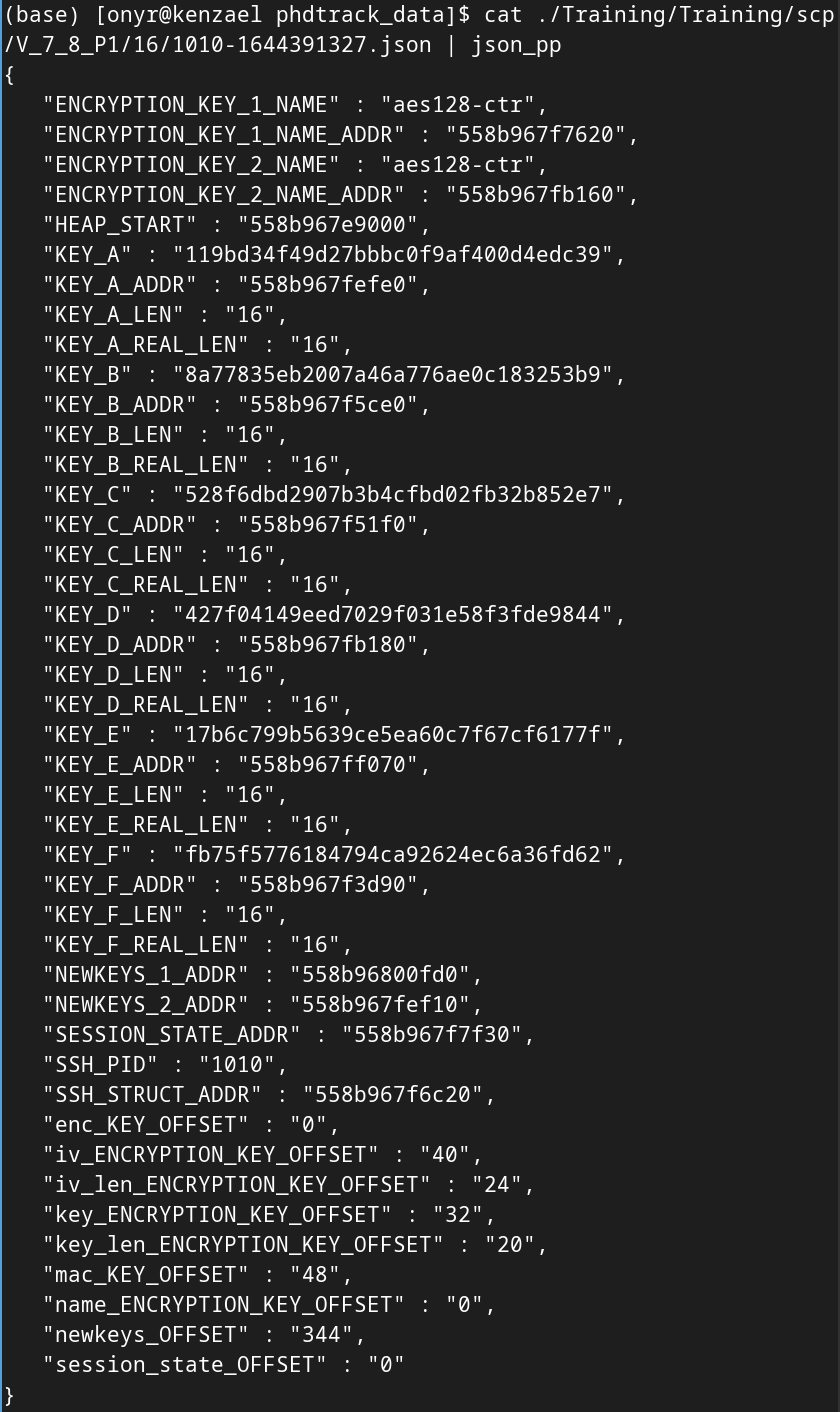
\includegraphics[width=0.6\textwidth]{img/background/json_annotation_for_1010-1644391327.png}
            \caption{Json exemple}
            \label{fig:Background:json}
        \end{figure}

        \begin{figure}[H]
            \centering
            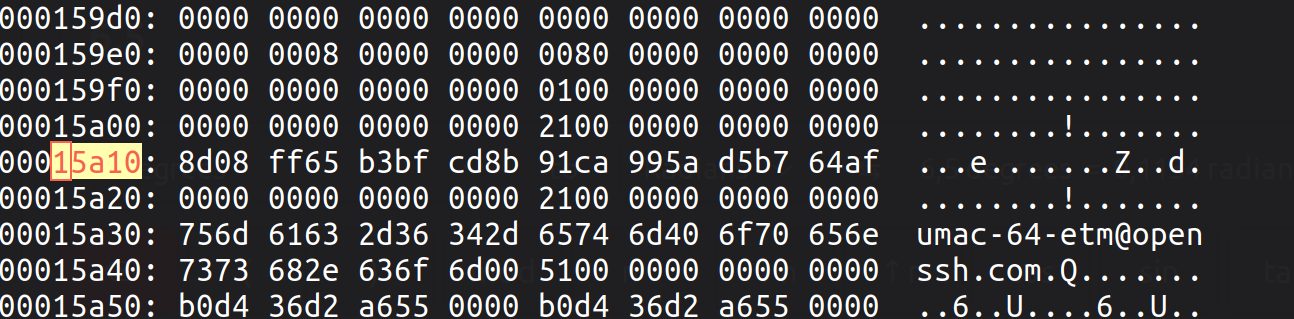
\includegraphics[width=0.6\textwidth]{img/background/xxd.png}
            \caption{Xxd exemple}
            \label{fig:Background:xxd}
        \end{figure}

        \paragraph{}The dataset is structured into two primary directories: \texttt{training} and \texttt{validation}. Each of these directories is further segmented into subdirectories reflecting the specific scenario, such as OpenSSH, port-forwarding, or secure copy (\acrshort{scp}).

        \paragraph{}Subdirectories under OpenSSH or SCP are categorized based on the software version responsible for the memory dump. These directories are further organized by the software version that generated the memory dump. The heaps are then classified based on their key lengths, with each key length possessing its dedicated directory beneath the version directory. These version-specific directories are further divided based on the different key lengths present in a heap.

        \paragraph{}Accompanying every raw memory dump is a JSON file, distinguished by the same alphanumeric sequence, barring the ``-heap'' suffix. This JSON file encapsulates various encryption keys and additional metadata, such as the process ID and the offset of the heap. Consequently, the dataset's utility is not confined to extracting session keys but also extends to identifying crucial data structures harboring sensitive information. The dataset, along with the associated code and tools, is open-sourced. The dataset is accessible via a Zenodo repository\footnote{\url{https://zenodo.org/record/6537904}}. The code can be found in a public GitHub repository\footnote{Link to the GitHub repository}.}
        
        \paragraph{}This data is the same as the data used in the paper titled \citetitle*{fellicious_smartkex_2022} \cite{fellicious_smartkex_2022}.
    
    \subsubsection{Entropy's Role in SSH Key Identification}

        \paragraph{}Encryption keys\cite*{fellicious_smartkex_2022} inherently consist of predominantly random byte sequences. This characteristic stems from the foundational principle of ensuring security through transparency, which guarantees their high entropy. The paper explores the nuances of pinpointing these keys in memory dumps, underscoring the significance of entropy in this endeavor. This particularity can be used to identify the keys in the memory dump.
        
    \subsubsection{Definitions : Structures, Pointers, and the role of malloc headers}
    
        \paragraph{}Through the use of the regular expressions (\acrshort{regex}) \texttt{"[0-9a-f]\{12\}0\{4\}"}, we identified potential \glspl{pointer} within the dump. This heuristic approach acts as a sieve, filtering the extensive data to spotlight possible \gls{pointer} candidates. Nonetheless, it's crucial to understand that while many \glspl{pointer} might be correctly pinpointed, some detected sequences may not be authentic \glspl{pointer}.

        \paragraph{}One notable characteristic of the heap dump is the \textit{malloc header} found at the start of allocated \glspl{structure}. This header, often the initial non-null bytes in a series, signifies the size of the following \gls{structure}. By sequentially reading the heap dump and identifying these headers, it becomes feasible to determine the dimensions and limits of every allocated \gls{structure}, thereby methodically dividing the heap dump into distinct \glspl{structure}.
        
\subsection{Traditional Statistical Embedding}

    \paragraph{}Within the domain of machine learning, how data is represented significantly impacts the performance of models. Even though traditional statistical embedding techniques have been around before many contemporary methods, they continue to be vital in readying data for machine learning endeavors. Rooted in statistical foundations, these techniques provide a methodical approach to transform raw data into concise and meaningful forms. In this subsection, we'll delve into the nuances of entropy and its role in byte sequence embedding, \acrfull{bfd}, and also highlight other classical statistical embedding methods pivotal in data representation for machine learning.
        
    \subsubsection{Entropy and its application in byte sequence embedding}
        \paragraph{}Entropy, a fundamental concept in information theory, quantifies the amount of uncertainty or randomness associated with a set of data. Introduced by Claude Shannon in his groundbreaking work \cite{shannon_mathematical_1948}, entropy serves as a measure of the average information content one can expect to gain from observing a random variable's value.

        \paragraph{}Mathematically, the entropy \(H(X)\) of a discrete random variable \(X\) with possible values \newline \(\{x_1, x_2, \ldots, x_n\}\) and probability mass function \(P(X)\) is given by:
        \begin{align}
            H(X) &= -\sum_{i=1}^{n} P(x_i) \log_2 P(x_i)
            \label{eq:shannon_entropy}
        \end{align}

        \paragraph{}Within the scope of identifying SSH keys, the significance of entropy cannot be understated. Byte sequences exhibiting high entropy typically reflect a multifaceted and varied informational content, traits that are synonymous with encryption keys, especially those in SSH. Sequences with pronounced entropy are often prime contenders for SSH keys due to their inherent randomness and lack of predictability, mirroring the attributes of robust security keys.

        \paragraph{}Fundamentally, entropy acts as a quantitative tool to evaluate the depth of information within data. When applied to SSH, it suggests that data sequences with elevated entropy levels have a heightened probability of correlating with secure keys. This positions entropy as an essential instrument for pinpointing and authenticating SSH keys.
    \subsubsection{Byte Frequency Distribution (BFD)}
        \paragraph{}In the complex world of raw byte embedding, \acrfull{bfd} and n-gram embedding stand out as essential methods, each bringing unique benefits to data representation. \acrshort{bfd} zeroes in on the distribution of individual byte values in a raw byte sequence. Analyzing these distributions allows for the identification of patterns that reflect the inherent nature of the data. This embedding technique becomes particularly relevant when assessing the randomness or structure of byte sequences, such as when detecting encrypted data or pinpointing specific file signatures.

        \paragraph{}On the other hand, n-gram embedding dives deeper into raw byte sequences. Instead of focusing solely on individual bytes, it captures patterns formed by sequences of 'n' consecutive bytes. This approach garners a wider range of contextual information from the raw byte data. For example, a trigram (3-gram) examines patterns formed by three sequential bytes, providing a richer representation than single byte values. Yet, a challenge with n-gram embedding is the potential for the output vector size to grow exponentially as 'n' increases, posing computational and storage issues, especially in real-time scenarios.
        
        \paragraph{}In the realm of raw byte embedding, both \acrshort{bfd} and n-gram techniques offer invaluable perspectives. While \acrshort{bfd} establishes a base representation centered on individual byte frequencies, n-gram embedding enhances it by spotlighting the complex relationships and patterns among consecutive bytes. Together, they form a robust arsenal for representing and analyzing raw byte data in a variety of applications.
    \subsubsection{Other traditional statistical embedding techniques}
        \paragraph{Mean Byte Value}The Mean Byte Value represents the average value of all bytes in a given sequence. It provides an insight into the central tendency of the byte values in the sequence. Mathematically, for a byte sequence \( B \) of length \( n \):
        \begin{equation}
        \text{Mean Byte Value} = \frac{1}{n} \sum_{i=1}^{n} B_i
        \label{eq:mean_byte_value}
        \end{equation}

        \paragraph{Mean Absolute Deviation (MAD)}MAD measures the average distance of each byte value from the mean, providing a sense of the dispersion or spread of the byte values around the mean. It is given by:
        \begin{equation}
        \text{MAD} = \frac{1}{n} \sum_{i=1}^{n} |B_i - \text{Mean Byte Value}|
        \label{eq:mad}
        \end{equation}

        \paragraph{Standard Deviation}Standard Deviation quantifies the amount of variation or dispersion in the byte sequence. A higher value indicates greater variability in the byte values. It is defined as:
        \begin{equation}
        \text{Standard Deviation} = \sqrt{\frac{1}{n} \sum_{i=1}^{n} (B_i - \text{Mean Byte Value})^2}
        \label{eq:standard_deviation}
        \end{equation}

        \paragraph{Skewness}Skewness\cite{wheeler_problems_2011} measures the asymmetry of the distribution of byte values around the mean. A positive value indicates a distribution that is skewed to the right, while a negative value indicates a distribution skewed to the left. It provides insights into the shape of the distribution of byte values. The Fisher’s skewness\cite{cain_univariate_2017} is :
        \begin{equation}
        \text{Skewness} = \frac{n}{(n-1)(n-2)} \sum_{i=1}^{n} \left( \frac{B_i - \text{Mean Byte Value}}{\text{Standard Deviation}} \right)^3
        \label{eq:skewness}
        \end{equation}

        \paragraph{Kurtosis}Kurtosis\cite{wheeler_problems_2011} measures the "tailedness" of the distribution of byte values. A higher kurtosis value indicates a distribution with heavier tails, while a lower value indicates lighter tails. It provides insights into the extremities of the distribution. The Fisher’s kurtosis\cite{cain_univariate_2017} is :
        \begin{equation}
        \text{Kurtosis} = \frac{n(n+1)}{(n-1)(n-2)(n-3)} \sum_{i=1}^{n} \left( \frac{B_i - \text{Mean Byte Value}}{\text{Standard Deviation}} \right)^4 - \frac{3(n-1)^2}{(n-2)(n-3)}
        \label{eq:kurtosis}
        \end{equation}

        \paragraph{n-gram on Bits}When applying n-gram techniques to bits instead of bytes, we focus on sequences of 'n' consecutive bits. For example, a 2-gram on bits would consider patterns formed by two consecutive bits, resulting in four possible combinations: 00, 01, 10, and 11. This approach significantly reduces the size of the output vector compared to byte-based n-grams. By focusing on bits, we can capture more granular patterns in the data while benefiting from a more compact representation, which is computationally efficient and requires less storage.

\subsection{Deep Learning Models for Raw Byte Embedding}

    \paragraph{}In the area of data representation, deep learning is great for understanding raw byte sequences. Just like these models are good at understanding text, they're also good at understanding raw bytes. They can learn and show sequences on their own, which is really helpful for both text and raw bytes. In this section, we'll look at different deep learning models and how they work with raw byte embedding.

    \paragraph{}We'll start with \acrfull{rnn}. Just like they're good with word sequences in text, \acrfull{rnn} are also good with raw byte sequences. Then, we'll look at \acrfull{cnn}, which can find patterns in raw bytes, just like they find patterns in text. After that, we'll talk about Autoencoders, which can learn in a special way. To finish this section, we'll discuss Transformers. They're good at understanding data over a long time, similar to how they understand text.

    \subsubsection{RNNs : Understanding sequence data}
        \paragraph{}\acrfull{rnn} are great tools for text classification. They're good at understanding the deeper meanings in text. Unlike older models that use hand-made features, \acrshort{rnn} can learn and show sequences on their own. This makes them really useful for tasks that deal with sequences. When we think about embedding raw bytes, \acrshort{rnn}'s skill in understanding sequences is similar to how they handle word sequences in text. Here is a list of different \acrshort{rnn} models and their advantages and disadvantages.

        \paragraph{\acrfull{rcnn} for Text Classification\cite{lai_recurrent_2015}:} The \acrshort{rcnn} model, as discussed in the paper by Lai et al., is designed specifically for text classification. Unlike traditional models, \acrshort{rcnn} do not rely on handcrafted features. Instead, they employ a recurrent structure to capture contextual information about words. This approach is believed to introduce considerably less noise compared to traditional window-based neural networks. The model's bidirectional structure ensures that both preceding and succeeding contexts of a word are considered, enhancing its understanding of the word's semantics.

        \begin{itemize}
            \item \textbf{Advantages:} 
            \begin{itemize}
                \item No need for handcrafted features.
                \item Captures richer contextual information.
                \item less noisy.
            \end{itemize}
            \item \textbf{Disadvantages:} 
            \begin{itemize}
                \item Complexity due to bidirectional structure.
                \item Might require more computational resources.
            \end{itemize}; 
        \end{itemize}

        \paragraph{\acrfull{lstm}\cite{hochreiter_long_1997}:}The \acrshort{lstm}, introduced by Hochreiter and Schmidhuber, is a specialized form of \acrshort{rnn} designed to combat the vanishing gradient problem inherent in traditional \acrshort{rnn}. The vanishing gradient problem arises when gradients of the loss function, which are used to update the network's weights, become too small for effective learning. This typically happens in deep networks or when processing long sequences, causing the earlier layers or time steps to receive minimal updates. As a result, traditional \acrshort{rnn} struggle to learn long-term dependencies in the data.

        \paragraph{}\acrshort{lstm} address this issue with their unique cell state and gating mechanisms. The cell state acts as a "conveyor belt" that can carry information across long sequences with minimal changes, ensuring that long-term dependencies are captured. The gating mechanisms, namely the input, forget, and output gates, regulate the flow of information into, out of, and within the cell. This design allows LSTMs to selectively remember or forget information, making them adept at learning and retaining long-term dependencies in sequences.

        \begin{itemize}
            \item \textbf{Advantages:}
            \begin{itemize}
                \item Efficiently learns long-term dependencies; overcomes the vanishing gradient problem inherent in traditional \acrshort{rnn}.
                \item Often achieves faster and more stable learning.
            \end{itemize}
            \item \textbf{Disadvantages:}
            \begin{itemize}
                \item More complex architecture compared to basic \acrshort{rnn} and even \acrshort{gru}.
                \item Can be computationally intensive due to the multiple gating mechanisms.
            \end{itemize}
        \end{itemize}

        \paragraph{\acrfull{gru}\cite{chung_empirical_2014}:} \acrshort{gru} are a variant of \acrshort{rnn} that aim to capture long-term dependencies without the complexity of \acrshort{lstm}. They use a gating mechanism to control the flow of information, making them efficient in sequence modeling tasks.

        \begin{itemize}
            \item \textbf{Advantages:} 
            \begin{itemize}
                \item Simplified structure compared to \acrshort{lstm}.
                \item Efficient in capturing long-term dependencies.
                \item Sometimes outperforms \acrshort{lstm}.
            \end{itemize}
            \item \textbf{Disadvantages:} 
            \begin{itemize}
                \item Still more complex than traditional \acrshort{rnn}.
                \item Might not always outperform \acrshort{lstm} in all tasks.
            \end{itemize}
        \end{itemize}
        

        \paragraph{}To sum it up, \acrshort{rnn} are good at understanding sequences and context. This makes them a good choice for embedding raw bytes. Just like they understand words based on the words around them, \acrshort{rnn} can find patterns in raw byte sequences, giving us a better understanding of the data.
    \subsubsection{CNNs : Pattern detection in raw bytes}
        \paragraph{}\acrfull{cnn}\cite{lecun_gradient-based_1998} are a specialized category of deep learning models adept at identifying patterns. Originally designed for visual data, their prowess extends to tasks like image and document recognition. Drawing inspiration from the human visual cortex's biological processes, \acrshort{cnn} are architected to autonomously and adaptively discern spatial feature hierarchies from inputs. This becomes particularly relevant when considering raw byte embedding, where the goal is to detect patterns in sequences of bytes. The CNN architecture boasts convolutional layers that perform operations on input data to capture localized patterns, and pooling layers that condense spatial dimensions while preserving crucial information. This layered approach enables \acrshort{cnn} to detect intricate patterns by progressively building on simpler foundational patterns. When applied to byte sequences or document recognition, \acrshort{cnn} excel, showcasing remarkable efficacy, especially in tasks like identifying patterns within raw byte sequences or recognizing handwritten content.

        \paragraph{}When tailored to \acrshort{cnn}, the \acrfull{seq2seq}\cite{gehring_convolutional_2017} approach emerges as a potent tool for transforming raw byte sequences into meaningful embeddings. The encoder segment of the \acrshort{seq2seq} model is central to this transformation. It delves into the byte sequence, discerning intricate patterns and nuances, and distills this rich information into a concise context vector or embedding. This condensed representation captures the core essence of the byte sequence, positioning it as a valuable input for subsequent tasks, such as classification models.

        \paragraph{}At the heart of the encoder lie the convolutional layers, skilled in pinpointing specific patterns within the byte sequence. Whether it's unique byte combinations or indicative n-grams, these layers are primed to detect them. As they traverse the raw byte sequence, they employ specialized filters, honed to recognize these specific patterns. As the data flows through the encoder's layers, these identified patterns are synthesized and refined, culminating in a comprehensive embedding of the sequence.

        \paragraph{}Here are two \acrfull{seq2seq} models using \acrshort{cnn} :
        

        \begin{itemize}
            \item \textbf{Autoencoders:} These neural network architectures\cite{hinton_reducing_2006} are designed for data compression and reconstruction. The encoder part compresses the input data into a compact representation, while the decoder reconstructs the original data from this representation. In the context of raw byte sequences, the encoder can be used to generate embeddings that capture the essential patterns and structures of the data.

            \item \textbf{Transformers :} Transformers\cite{vaswani_attention_2017} utilize self-attention mechanisms to weigh the significance of different parts of the input data. This allows them to capture long-range dependencies and relationships in the data. When applied to raw byte sequences, transformers can generate embeddings that consider both local and global patterns, making them particularly effective for tasks that require understanding the broader context of a sequence.

        \end{itemize}
        
        \paragraph{}Yet, a significant challenge with traditional \acrfull{seq2seq} models using \acrshort{cnn} is their constraint in managing inputs of varying sizes. Constructed with a set input size, they face difficulties when presented with sequences of diverse lengths, like raw byte sequences.

        \paragraph{}To address this limitation, various techniques have been employed to normalize the size of the input data. One of the most common methods is \textbf{padding}, where shorter sequences are filled with predefined placeholder values (often zeros) until they match the length of the longest sequence in the dataset. This ensures that all sequences fed into the model have a uniform length. Another approach is \textbf{bucketing}, where sequences of similar lengths are grouped together, minimizing the amount of padding required. Additionally, \textbf{truncation} can be used to shorten sequences that exceed a certain length, although this might result in the loss of some information. While these techniques enable \acrshort{cnn}-based \acrfull{seq2seq} models to handle variable-sized inputs, it's crucial to ensure that the preprocessing steps do not introduce noise or distort the inherent patterns and relationships within the raw byte sequences.
\subsection{Graph Embedding Methods}
    Wait Onyr

\subsection{Machine learning}
    \paragraph{}Machine learning, an integral part of artificial intelligence, revolves around designing algorithms and statistical models that allow computers to perform tasks without being directly programmed. Instead of relying on detailed instructions for every task, machine learning techniques empower systems to learn from data and make data-driven decisions. A key method in this field is supervised learning, in which models are trained using data that comes with predefined labels. Here, each piece of data in the training set has an associated known output. The primary goal of supervised learning is to establish a relationship between inputs and outputs, enabling the model to predict or categorize new, unseen data based on this relationship.

    \paragraph{}A cornerstone in this realm is feature engineering, which involves the meticulous process of selecting and transforming variables to optimize model performance. Another challenge frequently encountered by practitioners is dealing with datasets where some classes are overrepresented, which can skew model predictions. Among the myriad of machine learning models available, certain ones have gained prominence due to their versatility and effectiveness. We will provide an overview of some of these notable models.

    \subsubsection{Features engineering}
        \paragraph{}Feature engineering\cite{khurana_feature_2017} is a cornerstone in the realm of machine learning. It involves the artful transformation of the given feature space to optimize the performance of predictive models. The significance of feature engineering cannot be overstated; it serves as a bridge between raw data and the predictive models, ensuring that the models are fed with the most relevant and informative features. Properly engineered features can drastically reduce modeling errors, leading to more accurate and reliable predictions. Here are some of the most common feature engineering techniques:

        \begin{itemize}
            \item \textbf{Normalization and Scaling }are preprocessing techniques used to standardize the range of independent features in the data. Many machine learning algorithms, especially those that rely on distance calculations like k-means clustering or support vector machines, are sensitive to the scale of the data. If features are on different scales, one feature might dominate others, leading to suboptimal model performance. Normalization typically scales features so that they have a unit norm, while other scaling methods, such as Min-Max scaling, transform features to lie in a given range, usually [0,1]. Z-score normalization or standard scaling is another method where features are scaled based on their mean and standard deviation. Properly scaled data ensures that each feature contributes equally to the model's decision, leading to more stable and accurate predictions.

            \item \textbf{Interaction Features\cite{khalid_survey_2014} }refer to the creation of new features by combining two or more existing features, aiming to capture any synergistic effect between them. In many cases, the interaction between variables can provide more information than the individual variables themselves. For instance, while analyzing real estate prices, the individual features 'number of rooms' and 'location' might be informative, but their interaction, 'number of rooms in a specific location', might offer even more predictive power. Interaction features can be created by multiplying, adding, or even dividing original features, and they can help in capturing non-linear relationships in the data, enhancing the model's ability to make accurate predictions.

            \item \textbf{Feature Selection\cite{khalid_survey_2014} }is a critical process in the machine learning pipeline that focuses on selecting the most relevant features from the original set, aiming to reduce the dimensionality and improve model performance. The primary goal is to eliminate redundant or irrelevant features that don't contribute significantly to the predictive power of the model. This not only helps in reducing the computational cost but also can lead to a more interpretable model. There are various techniques for feature selection, including filter methods (based on statistical measures), wrapper methods (like recursive feature elimination), and embedded methods (where algorithms inherently perform feature selection, such as decision trees). By judiciously selecting features, one can build efficient models that are less prone to overfitting and have better generalization capabilities.
        \end{itemize}

        \paragraph{}Following the aforementioned techniques, another essential facet in the feature engineering landscape is dimensionality reduction. As data grows in complexity, it often encompasses a vast number of features, leading to what is known as a high-dimensional space. While a plethora of features might seem advantageous, it introduces challenges, notably the \textit{curse of dimensionality}\cite{hutchison_curse_2005, koppen_curse_2000}. In such high-dimensional realms, data points tend to become increasingly sparse. This sparsity means that the relative distances between data points start to appear uniform, making it arduous for algorithms to discern meaningful patterns. This can lead to models that overfit the training data, capturing noise rather than the underlying data distribution. Additionally, the computational overhead increases, and deriving intuitive insights from the data becomes a daunting task.

        \paragraph{}Dimensionality reduction techniques come to the rescue by striving to trim down the number of features while preserving the crux of the information. Techniques like \acrfull{pca} and \acrfull{t-sne} are employed to transform the data from its original high-dimensional space to a more manageable, lower-dimensional one. This transformation aims to retain the significant patterns and structures inherent in the data. By judiciously reducing the dimensionality, not only can models be trained more efficiently, but they often yield better performance by focusing on the most pertinent features. This streamlined approach mitigates the challenges posed by the curse of dimensionality, ensuring models that are both robust and interpretable.

    \subsubsection{Imbalanced data}
        \paragraph{}In machine learning, a frequent obstacle is the presence of datasets where one category vastly overshadows others\cite{ramyachitra_imbalanced_2014}. This imbalance can skew models towards predicting the dominant class, often neglecting the less prevalent but potentially more critical class.

        \paragraph{}To counteract this, a variety of techniques have been devised:
        \begin{itemize}
            \item \textbf{Resampling:} This encompasses both increasing instances of the minority class (oversampling) and decreasing instances of the majority class (undersampling). A notable method for oversampling is the \acrfull{smote}, which generates artificial data points in the feature space.
            \item \textbf{Weighted Loss:} This strategy involves assigning greater weights to the minority class during the training phase, ensuring the model gives it due consideration.
            \item \textbf{Ensemble Methods:} Approaches such as bagging and boosting can be tailored to ensure a balanced class representation. For example, in bagging, each sample can be structured to maintain a balanced class ratio.
            \item \textbf{Anomaly Detection:} This method reframes the task from classification to anomaly detection, viewing the minority class as an outlier or anomaly.
        \end{itemize}
        \paragraph{}Selecting an appropriate strategy hinges on the specific problem and dataset characteristics. It's also crucial to evaluate the model's efficacy using suitable metrics, ensuring it genuinely addresses the imbalance.

    \subsubsection{Some common models}
    \begin{itemize}
        \item \textbf{Logistic Regression\cite{nick_logistic_2007} : }Logistic regression serves as a statistical technique tailored for binary classification tasks. While linear regression is designed to forecast continuous outcomes, logistic regression focuses on predicting the likelihood of a binary result. It leverages the logistic function to relate multiple independent variables to a binary outcome, ensuring the predicted values fall between 0 and 1. Typically, a 0.5 threshold is used to classify the final outcome. A key strength of logistic regression is its clarity and ease of interpretation, though it might face challenges with complex non-linear data unless further feature adjustments are made.
        
        \item \textbf{Decision Trees\cite{kotsiantis_decision_2013} : }Decision trees are machine learning models designed for both classification and regression tasks. They segment data into subsets based on feature values, making decisions at each node. While their hierarchical structure offers easy visualization and interpretation, they can be prone to overfitting. However, strategies like pruning can help in refining the tree and mitigating overfitting.
        
        \item \textbf{Random Forest\cite{probst_hyperparameters_2019} : }Random Forest is an ensemble method that creates a 'forest' of decision trees. Each tree is trained on a random subset of the data and makes its own predictions. The Random Forest algorithm then aggregates these predictions to produce a final result. This method is known for its high accuracy, ability to handle large datasets with higher dimensionality, and its capacity to manage missing values.
        
        \item \textbf{\acrfull{svm}\cite{wu_analysis_2006} : }\acrshort{svm} are used for both regression and classification problems. They work by finding the hyperplane that best divides a dataset into classes. SVMs are effective in high-dimensional spaces and are versatile, as different Kernel functions can be specified for the decision function.
        
        \item \textbf{\acrfull{knn}\cite{laaksonen_classification_1996} :}\acrshort{knn} is a simple, instance-based learning algorithm. To make a prediction for a new data point, the algorithm finds the 'k' training examples that are closest to the point and returns the most common output value among them.
    \end{itemize}